\documentclass[border=2pt]{standalone}
\usepackage[T1]{fontenc}
\usepackage[scaled=1.0]{helvet}
\renewcommand{\familydefault}{\sfdefault}
\usepackage{sfmath}
\usepackage{amsmath}
\usepackage{xcolor}
\usepackage{tikz}
\usetikzlibrary{positioning,arrows.meta,calc,fit,backgrounds,shapes.geometric}
% palette (light fills, dark strokes: prints well in colour and greyscale)
\definecolor{ink}{HTML}{1F2933}
\definecolor{muted}{HTML}{52606D}
\definecolor{dataS}{HTML}{B7791F}\definecolor{dataF}{HTML}{FDF3E1}
\definecolor{physS}{HTML}{2F6DB5}\definecolor{physF}{HTML}{E6EFFA}
\definecolor{tranS}{HTML}{2E7D4F}\definecolor{tranF}{HTML}{E5F4EA}
\definecolor{repS}{HTML}{6B4FA8}\definecolor{repF}{HTML}{EFEAF8}
\definecolor{greyS}{HTML}{7B8794}\definecolor{greyF}{HTML}{F1F3F5}
\tikzset{
  >={Stealth[length=2.6mm,width=2mm]},
  box/.style={draw, rounded corners=2pt, line width=0.7pt, align=center, inner sep=4pt, text=ink},
  ttl/.style={font=\bfseries\small},
  arr/.style={->, line width=0.9pt, draw=ink},
  darr/.style={->, line width=0.8pt, draw=muted, dashed},
  stage/.style={draw, rounded corners=4pt, line width=0.6pt, dash pattern=on 3pt off 2pt, inner sep=7pt},
  stagelabel/.style={font=\bfseries\small, anchor=south west, inner sep=2pt},
}
\usepackage[none]{hyphenat}
\newcommand{\T}[1]{{\small\bfseries #1}\\[1pt]}

\begin{document}
\footnotesize
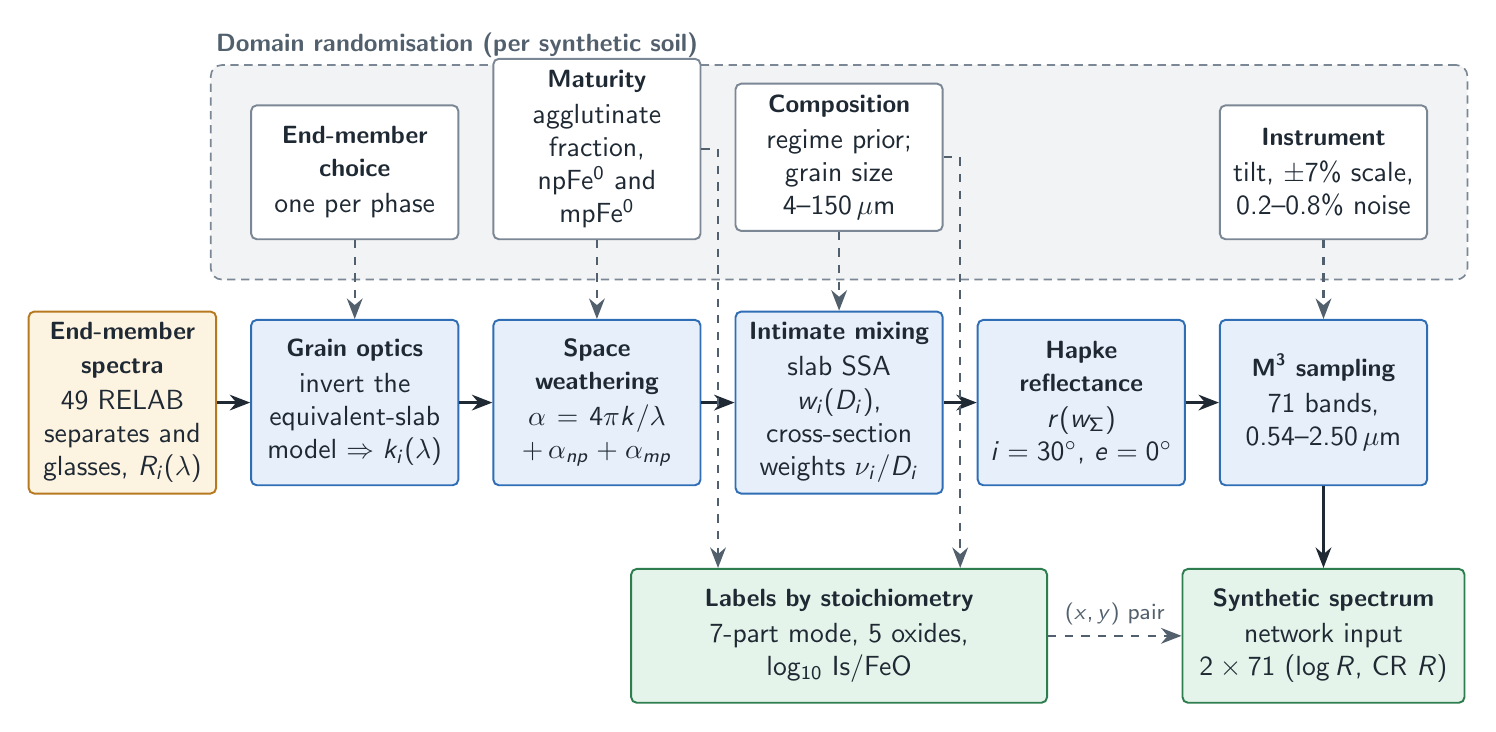
\begin{tikzpicture}[node distance=5mm and 4.2mm]
\tikzset{chain/.style={box, draw=physS, fill=physF, text width=23.5mm, minimum height=21mm},
         rnd/.style={box, draw=greyS, fill=white, text width=23.5mm, minimum height=17mm}}
% main chain
\node[box, draw=dataS, fill=dataF, text width=21mm, minimum height=21mm] (em) {\T{End-member spectra}49 RELAB\\separates and\\glasses, $R_i(\lambda)$};
\node[chain, right=of em] (opt) {\T{Grain optics}invert the\\equivalent-slab\\model $\Rightarrow k_i(\lambda)$};
\node[chain, right=of opt] (sw) {\T{Space weathering}$\alpha = 4\pi k/\lambda$\\$+\,\alpha_{np} + \alpha_{mp}$};
\node[chain, right=of sw] (mix) {\T{Intimate mixing}slab SSA $w_i(D_i)$,\\cross-section\\weights $\nu_i/D_i$};
\node[chain, right=of mix] (hap) {\T{Hapke reflectance}$r(w_{\Sigma})$\\$i=30^\circ$, $e=0^\circ$};
\node[chain, right=of hap] (smp) {\T{M\textsuperscript{3} sampling}71 bands,\\0.54--2.50\,$\mu$m};
% randomisation row
\node[rnd, above=10mm of opt] (r1) {\T{End-member choice}one per phase};
\node[rnd, above=10mm of sw] (r2) {\T{Maturity}agglutinate fraction,\\npFe$^0$ and mpFe$^0$};
\node[rnd, above=10mm of mix] (r3) {\T{Composition}regime prior;\\grain size\\4--150\,$\mu$m};
\node[rnd, above=10mm of smp] (r4) {\T{Instrument}tilt, $\pm$7\% scale,\\0.2--0.8\% noise};
% outputs
\coordinate (g1) at ($(sw.east)!0.5!(mix.west)$);
\coordinate (g2) at ($(mix.east)!0.5!(hap.west)$);
\node[box, draw=tranS, fill=tranF, text width=50mm, minimum height=17mm, anchor=north] (lab) at ($(g1)!0.5!(g2)+(0,-21mm)$) {\T{Labels by stoichiometry}7-part mode, 5 oxides,\\log$_{10}$ Is/FeO};
\node[box, draw=tranS, fill=tranF, text width=33mm, minimum height=17mm] (syn) at (lab.east -| smp.center) {\T{Synthetic spectrum}network input\\$2\times71$ ($\log R$, CR $R$)};
\draw[arr] (em) -- (opt); \draw[arr] (opt) -- (sw); \draw[arr] (sw) -- (mix); \draw[arr] (mix) -- (hap); \draw[arr] (hap) -- (smp);
\draw[arr] (smp.south) -- (smp.south |- syn.north);
\foreach \a/\b in {r1/opt, r2/sw, r3/mix, r4/smp} \draw[darr] (\a) -- (\b);
\draw[darr] (r2.east) -| (g1 |- lab.north);
\draw[darr] (r3.east) -| (g2 |- lab.north);
\draw[darr] (lab.east) -- node[above, font=\footnotesize, text=muted]{$(x, y)$ pair} (syn.west);
\begin{scope}[on background layer]
\node[stage, draw=greyS, fill=greyF, fit=(r1)(r4), inner sep=5mm] (dr) {};
\end{scope}
\node[stagelabel, text=muted] at (dr.north west) {Domain randomisation (per synthetic soil)};
\end{tikzpicture}
\end{document}
